%\newpage
  \begin{titlepage}
    \vspace*{\fill}
      \part{Introduction}
    \vspace*{\fill}
  \end{titlepage}

%\chapter{Introduction}\label{ch:introduction}
\phantomsection
\chapter*{Contents}

\textit{The main motive of this project is to understand real-time facial expression recognition systems and their applications. Then a review of the architecture of such systems will be done, along with a state of the art of already existing algorithms for each step. After this study, one algorithm for each step will be chosen, considering their difficulty and their efficiency, in order to improve it. In the last part, the problem will be formulated.}
\pagebreak

\phantomsection
\chapter{Motivations}

A facial expression is a visible manifestation of the effective state, cognitive activity, intent, personality, and psychopathology of a person \cite{DON99}; facial expressions play a significant role in human dialogue and interaction. Indeed, facial expressions carry more informations than mere speech, informations on which humans can relay for interaction. Facial expressions have a considerable effect on a listening interlocutor; a speaker facial expressions accounts for about 55 percent of the effect, 38 percent of the latter is conveyed by voice intonation and 7 percent by the spoken words \cite{PAN00}.
\newline

\noindent Since Antiquity, researchers have been interested in emotion and more particularly in emotion recognition. But one of the important studies on facial expression analysis impacting on the modern day science of automatic facial expression recognition was the work carried out by Charles Darwin \cite{BET12}. In 1872, Darwin wrote a treatise that established general expression principles and expression means for both humans and animals \cite{DAR04}. He also classified various kinds of expressions. This can be considered as the beginning of facial expression recognition.
\newline

\noindent Now, with the emergence of new technologies and computers, research is now focused on computer-based automatic facial expression recognition. Because facial expressions are major factors in human interaction, this research field will broaden the domain of Human-Machine Interaction. Indeed, emotion recognition will enable computers to be more responsive to users' emotions, and allow interactions to become more and more realistic. 
\newline

\noindent Another domain where facial expression recognition is an important issue is robotics. With the advances made in robotics, robots nowadays tend to mimic human emotion and react as as human-like as possible, especially for humanoid robots. However, since robots are being more and more present in our daily lives, they need to understand and recognize human emotions.
\newline

\noindent There are also various other domains where emotion recognition can be used: Telecommunications, behavioral science, video games, animations, psychiatry, automobile safety, affect-sensitive music juke boxes and televisions, educational software, etc \cite{BET12}.
\newline

\noindent A lot of real time applications have already been created. For example, Bartlett et al. have successfully used their face expression recognition system to develop an animated character that mirrors the expressions of the user (called CU Animate) \cite{BAR03}. They have also been successful in deploying the recognition system on Sony's Aibo Robot and ATR's RoboVie \cite{BAR03}. Another interesting application has been demonstrated by Anderson and McOwen, called "EmotiChat" \cite{AND06}. It is a regular chatroom, except the fact that their facial expression recognition system is connected to the chat and convert the users' facial expressions into emoticons. Because facial expression recognition systems' robustness and reliability are constantly increasing, lots of innovative applications will appear.
\newpage

\phantomsection
\chapter{Facial expression recognition}

\phantomsection
\section{General structure}

\noindent Facial expression eecognition is a system enabling an automatic recognition of emotions displayed by a human face. Facial expression recognition can be image or video-based; it can also be computed real-time. Most of the time, researchers try to recognize emotions ou of images of human faces. This can also be achieved real-time on video streams : While the person displays his/her emotions, the facial expression recognition system analyzes the video, and detect in real-time the displayed emotion.
\newline

\noindent In both cases, facial expression recognition process is structured as follows:


\noindent 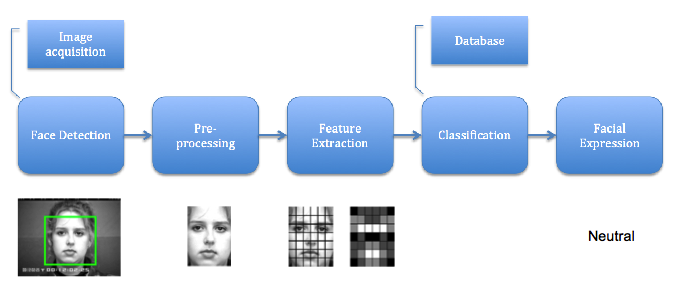
\includegraphics[scale=0.6]{figures/facial_expression_recognition_process}

\noindent First step of the process is "Image Acquisition". Images used for facial expression recognition can be static images or image sequences. Image sequences give more informations about the facial expression, as the steps in muscles movement. About static images, facial expression recognition systems usually need 2D greyscale images as inputs. We can however expect future systems to use colour images; first because of the increasing affordability of technologies and devices capable of capturing images or image sequences; then because colours can give more information on emotions, i.e blushing \cite{CHI03}.
\newline

\noindent Second step is "Face Detection". Indeed, in a static image and even more in an images sequence, this is an obvious need. Once the face has been detected, all other non-relevant information can be deleted, since only the face is needed. It could hence be included in the next step, which is "Pre-processing", but because of its importance it represents a step in itself. In a real-time facial expression recognition system working with image sequences, the face has to be detected, but also tracked. One of the most used and famous detection and tracking algorithm is the Viola-Jones Algorithm, which we will explain in detail later in ths report. This algorithm can be trained to detect all kind of objects, but is mostly used for face detection. 
\newline

\noindent Third step is "Pre-processing", which is about applying image processing algorithms to the image, in order to prepare it for the next step. Pre-processing is usually about noise removal, normalization against the variation of pixel position or brightness, segmentation, location, or tracking of parts of the face. Emotion recognition is also sensitive to transformation, scaling and rotation of the head in the image or image sequence. In order to solve this problem, the image can be geometrically standardized. References used for this standardization are usually the eyes \cite{CHI03}.
\newline

\noindent Once the image has gone through the "Pre-processing" step, the next one is "Features Extraction". In this step, data is converted into a higher representation of shape, motion, colour, texture, and spatial configuration of the face or its components. One of the main goals of this step is to reduce the dimensionality of the input data. The reduction procedure should retain essential information possessing high discrimination power and high stability \cite{CHI03}. There are a lot of features extraction methods. The most famous are : Principal Component Analysis (PCA), Linear Discriminant Analysis (LDA), Problem Based Learning (PBL), Hidden Markov Model (HMM), Eigenfaces, Gabor Wavelets. The extracted data is then used in the "Classification" step.
\newline

\noindent
\textbf{\color{red} INSERT PARAGRAPH ON CLASSIFICATION}

\phantomsection
\section{Existing systems}

\noindent Principal Component Analysis (PCA) : Principal Component Analysis is a statistical method; one of the most used in linear algebra. PCA is mainly used to reduce high dimensionality of data and to obtain the most important information from this data. Because Facial Expression Recognition needs to reduce the dimensionality of data during features extraction, PCA is commonly used. It helps transforming high dimensionality of data to a new coordinate system of lower dimensions while still preserving the most important information. PCA computes a covariance matrix and a set of values called the eigenvalues and eigenvectors from the original data \cite{GAN08}.
\newline

\noindent Linear Discriminant Analysis (LDA) : Linear Discriminant Analysis is a statistical method as PCA, used to classify a set of objects into groups. It is done by observing a set of features that describe the objects. LDA as PCA are used to establish a linear relationship between the dimensions of the data. The main difference is that LDA uses the linear relationship to model the differences into classes of objects and PCA does not take any differences into account in the linear relationship. The idea is to perform a linear transformation on the data to obtain a lower dimensional set of features \cite{GAN08}.
\newline

\noindent Problem Based Learning (PBL) : Problem Based Learning is a features extraction method with an appearance based approach. It can be used to describe texture and shape. PBL extracts some informations from the neighborhood of a central pixel. It compares the intensity values of the neighborhood pixels with the intensity value of the central pixel  \cite{GAN08}.
\newline

\noindent Hidden Markov Model (HMM)
\newline
\noindent Eigenfaces
\newline
\noindent Gabor Wavelets
\newline

\phantomsection
\section{Issues}

\noindent bla bla bla
\newline

\phantomsection
\section{Requirements}

\noindent bla bla bla
\newline









\noindent Before developing a facial expression recognition project, it is important to know what already exist; the state of the art of facial expression recognition system. In this chapter, an overview will be given of the existing systems before to decide on a system for the project.
\newline
